The inclusion of Scorched Land Defense as the target video game seems rather pointless as everyone was allowed to make \textit{any} video game they wanted to.
If the goal is supposed to be the creation of some specific video game or program, it should be defined in less vague terms than Scorched Land Defense was.


We were unable to flash the SD Card on the lab computers.
While attempting to compile the Linux kernel we also encountered way more problems than the distributed guidelines and exercise lectures had us believe it'd be.


The ``defense'' in ``Scorched Land Defence'' is spelled inconsistently in the provided material.
In the compendium it is spelled with a `s' on two occasions (in section 4) and `c' on six occasions (in the preface and throughout section 1).
In the Lab Introduction Lecture and the Exercise 3 Lecture it is spelled with a `c'.
Unsure if the two occurrances of `s' are typos or not, we have written it as ``defense'' roughly one out of three times throughout our work.


The measure of work spent on the assignment has steadily increased throughout the semester. See figure~\ref{img-commitgraphs}.

\begin{figure}[h!]
	\centering
	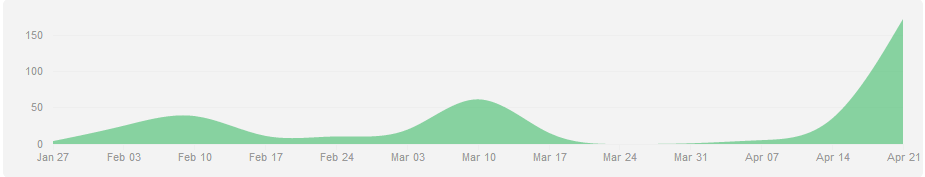
\includegraphics[width=6in]{{images/graph-commits.png}}
	\caption{A graph of contributions to the github repository over time.}
	\label{img-commitgraphs}
\end{figure}